%MAGIC COMMANDS
% !TeX TXS-program:compile = txs:///arara
% arara: lualatex: {shell: no, synctex: yes, interaction: batchmode}
% arara: pythontex: {rerun: modified} if exists('pytxcode') && found('pytxcode', 'PYTHONTEX#py')
% arara: lualatex: {shell: no, synctex: yes, interaction: batchmode} if exists('pytxcode') && found('pytxcode', 'PYTHONTEX#py')
% arara: lualatex: {shell: no, synctex: yes, interaction: batchmode} if found('log', '(undefined references|Please rerun|Rerun to get)')

\documentclass[a4paper,11pt]{article}
\usepackage[revgoku]{cp-base}
\graphicspath{{./graphics/}}
%variables
\donnees[%
	classe=1\up*{ère} 2M2,
	matiere={[SPÉ.MATHS]},
	mois=Juin,
	typedoc=CAHIER DE VACANCES,
	numdoc=1
]

%formatage
\author{Pierquet}
\title{\nomfichier}
\hypersetup{pdfauthor={Pierquet},pdftitle={\nomfichier},allbordercolors=white,pdfborder=0 0 0,pdfstartview=FitH}
%fancy
\lhead{\entete{\matiere}}
\chead{\entete{\lycee}}
\rhead{\entete{\classe{} - \mois{} \annee}}
\lfoot{\pied{\matiere}}
\cfoot{\logolycee{}}
\rfoot{\pied{\numeropagetot}}

%divers

\begin{document}

\pagestyle{fancy}

\part*{En route vers la Terminale (Correction)}

\newcommand\htimg{2.1cm}

\smallskip

\exogen{ A1}

\begin{enumerate}
	\item La suite $\suiten$ est définie de manière explicite :
	\begin{itemize}
		\item $u_0 = 2\times0^2-0+1=1$ ;
		\item $u_1 = 2\times1^2-1+1=2$ ;
		\item $u_2 = 2\times2^2-2+1=7$.
	\end{itemize}
	\item La suite $\suiten[v]$ est définie par récurrence :
	\begin{itemize}
		\item $v_1=-2$ ;
		\item $v_2 = \dfrac{1-v_0}{1} = \dfrac{1-(-2)}{1}=3$ ;
		\item $v_3 = \dfrac{1-v_1}{2} = \dfrac{1-3}{2}=-1$.
	\end{itemize}
	\item La suite $\suiten[w]$ est définie par récurrence :
	\begin{itemize}
		\item $w_0=5$ ;
		\item $w_1 = 2w_0-1=2\times5-1=9$ ;
		\item $w_2 = 2w_1-1=2\times9-1=17$.
	\end{itemize}
	\item La suite $\suiten[t]$ est définie de manière explicite :
	\begin{itemize}
		\item $t_0=3\big(1+(-1)^0\big)+2=3(1+1)+2=8$ ;
		\item $t_1=3\big(1+(-1)^1\big)+2=3(1-1)+2=2$ ;
		\item $t_2=3\big(1+(-1)^2\big)+2=3(1+1)+2=8$.
	\end{itemize}
\end{enumerate}

\medskip

\exogen{ A2}

\begin{enumerate}
	\item 
	\begin{enumerate}
		\item Par définition, on a $u_{n+1}=u_n+r=u_n-3$ et $u_n=u_0+\times r = 2-3n$ pour tout entier $n$.
		\item De ce fait, $u_{1000}=2-3\times1000=-2998$.
	\end{enumerate}
	\item 
	\begin{enumerate}
		\item On reconnaît $v_n = 4 \times 0,5^n = v_0 \times q^n$ donc $\suiten[v]$ est géométrique de 1\up{er} terme $v_0=4$ te de raison $q=0,5$.
		\item Par définition, $v_{n+1}=v_n\times q = v_n \times 0,5$ pour tout $n$.
		\item On a $S=v_0+v_1+\ldots+v_{10} = v_1 \times \dfrac{1-q^{11}}{1-q}=4 \times \dfrac{1-0,5^{11}}{1-0,5} \approx 7,996$ au millième.
	\end{enumerate}
\end{enumerate}

\medskip

\exogen{ A3}

\begin{enumerate}
	\item On a $u_1 = 500 \times \left(1+\frac{2}{100}\right) = 500 \times 1,02 = 510$ (prime la 2\up{ème} année).
	
	Et $u_2 = 510 \times 1,02 = 520,2$ (prime la 3\up{ème} année).
	\item On a directement le fait que $u_{n+1}=u_n \times 1,02$ pour tout entier $n$, ce qui justifie que la suite $\suiten$ est géométrique de raison $q=1,02$ et de 1\up{er} terme $u_0=500$.
	\item De ce fait, $u_n=u_0 \times q^n = 500 \times 1,02^n$ pour tout entier $n$.
	\item La raison $q$ étant strictement supérieure à 1, on a déjà le fait que $\left(1,02^n\right)$ est strictement croissante.
	
	Sachant que $u_0=500>0$, on en déduit que $\suiten$ est monotone croissante.
	\item 
	\begin{enumerate}
		\item La prime touchée la 20\up{ème} année est donnée par $u_{19}$, et $u_{19}=500 \times 1,02^{19} \approx 728,41$, soit 728,41\,€.
		\item La somme totale $S$ des primes touchées sur les 20 années est $S=u_0+u_1+\ldots+u_{19}$.
		
		Et $S=u_0 \times \dfrac{1-1,02^{20}}{1-1,02} \approx \num{11420,28}$ soit environ \num{11420,28}\,€.
	\end{enumerate}
\end{enumerate}

\pagebreak

\exogen{ A4}

\medskip

Le menu \ccalg{Suites} (ou un tableur\ldots) permet de conjecturer que $\lim_{n \to +\infty} t_n = -24$.

\begin{center}
	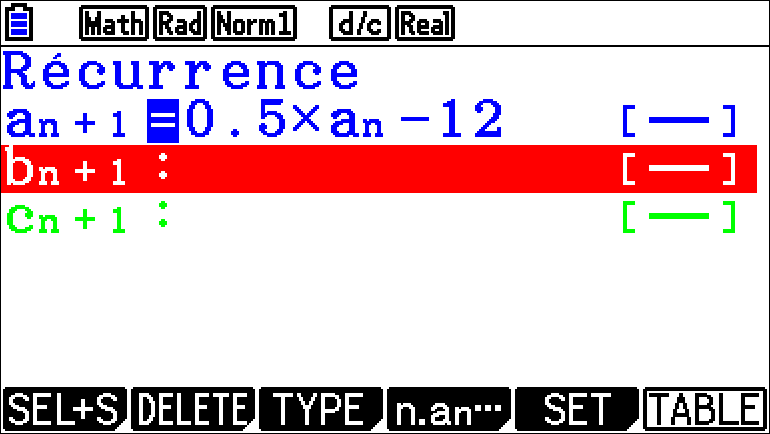
\includegraphics[height=\htimg]{roadterm_a4_a}~~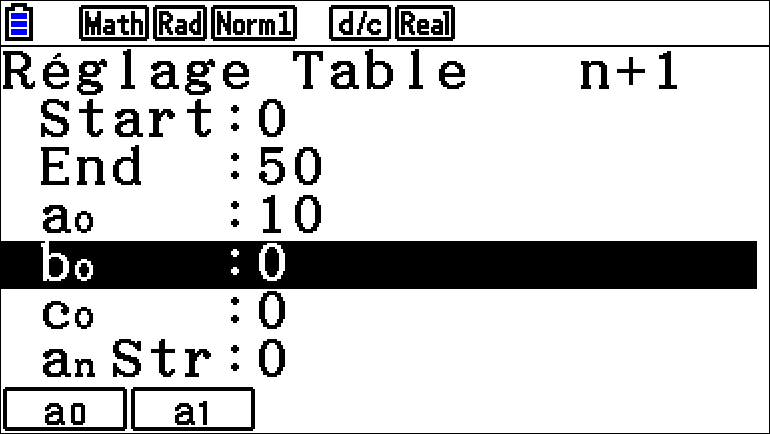
\includegraphics[height=\htimg]{roadterm_a4_b}~~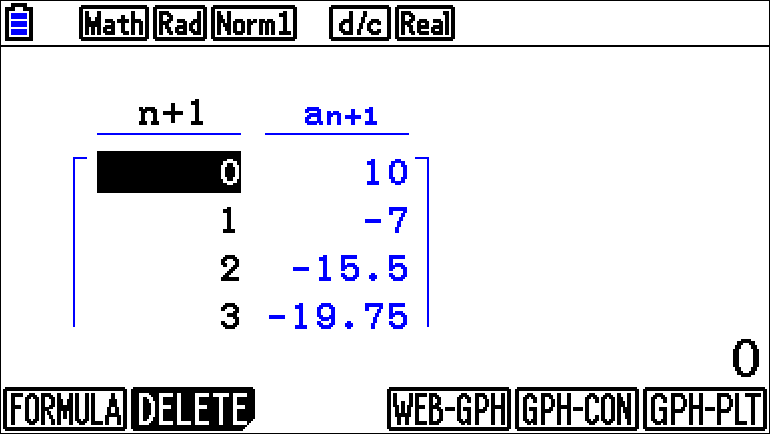
\includegraphics[height=\htimg]{roadterm_a4_c}~~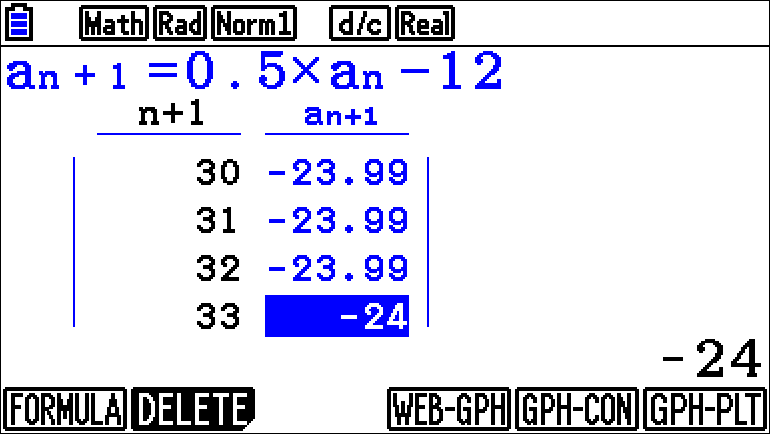
\includegraphics[height=\htimg]{roadterm_a4_d}
\end{center}

\medskip

\exogen{ A5}

\begin{enumerate}
	\item On a $u_{n+1}-u_{n} = \dfrac{1}{(n+1)(n+1+1)}-\dfrac{1}{n(n+1)}=\dfrac{1}{(n+1)(n+2)}-\dfrac{1}{n(n+1)}=\dfrac{n}{n(n+1)(n+2)}-\dfrac{n+2}{n(n+1)(n+2)}$.
	
	Soit encore $u_{n+1}-u_{n} = \dfrac{n-(n+2)}{n(n+1)(n+2)}=\dfrac{-2}{n(n+1)(n+2)}<0$ pour tout $n$ non nul.
	
	De ce fait $\suiten$ est monotone décroissante.
	\item Comme $n>0$ et $n+1>0$, alors $\dfrac{1}{n(n+1)}>0$ donc tous les termes de $\suiten$ sont strictement positifs.
	
	Et $\dfrac{u_{n+1}}{u_n}=\dfrac{\tfrac{1}{(n+1)(n+2)}}{\tfrac{1}{n(n+1)}}=\dfrac{1}{(n+1)(n+2)}\times \dfrac{n(n+1)}{1} = \dfrac{n}{n+2}<1$ pour tout $n\neq0$ (car $n<n+2$).
	
	De ce fait $\suiten$ est monotone décroissante.
	\item La fonction $f$ telle que $u_n = f\big(u_n\big)$ est ici $f(x)=\dfrac{1}{x(x+1)}=\dfrac{1}{x^2+x}$.
	
	La fonction $f$ est dérivable et $f'(x)=\dfrac{0\times(x^2+x)-(2x+1)\times1}{(x^2+x)^2}=\dfrac{-2x-1}{(x^2+x)^2}$ pour tout $x$ non nul.
	
	Ainsi on a $f'(x)<0$, ce qui donne le fait que $\suiten$ est monotone décroissante.
\end{enumerate}

\medskip

\exogen{ A6}

\begin{enumerate}
	\item $2x^2-2x-12=0$ est une équation du 2\up{nd} degré, avec $\Delta=100$ et les deux solutions sont $\begin{dcases} x_1 = 3 \\ x_2 = -2 \end{dcases}$.
	\item $-x^2+x=-2 \ssi -x^2+x+2=0$ qui est une équation du 2\up{nd} degré, avec $\Delta=9$ et les deux solutions $x_1=-1$ et $x_2=2$.
	\item $3x^2+x\sqrt{12}+1=0$ est une équation du 2\u{nd} degré (avec $b=\sqrt{12}$ !), avec $\Delta=0$ et la solution $x_0=-\dfrac{\sqrt{3}}{2}$.
	\item $4x^2+16=0$ est une équation du 2\up{nd} degré, avec $\Delta=-256$ donc pas de solution.
	\item $x^2+x=0 \ssi x(x+1)=0$ qui est une équation produit, avec comme solutions $x=0$ ou $x=-1$.
	\item $\big(x^2+5x+6\big)\big(x^2+x+1\big)=0$ est une équation produit :
	\begin{itemize}
		\item $x^2+5x+6=0$ : $\Delta=1$ et les solutions sont $x_1=-3$ et $x_2=-2$ ;
		\item $x^2+x+1=0$ : $\Delta=-3$ donc pas de solution.
	\end{itemize}
	Les solutions sont donc $\mathscr{S} = \ensPL[\strut]{-3 / -2}$.
\end{enumerate}

\pagebreak

\exogen{ A7}

\begin{enumerate}
	\item $4x-7$ est une expression du premier degré, avec $m=4\oplus$ et $4x-7=0 \ssi x=\nicefrac{7}{4}$ :
	
	\begin{center}
		\begin{tikzpicture}
			\tkzTabInit{$x$/0.8,expr/0.8}{$-\infty$,$\nicefrac{7}{4}$,$+\infty$}
			\tkzTabLine{,-,z,+,}
			\aidesignetkztabPL[code=da+,racines={7/4},couleur=orange]{1}[0.75][1.5]
		\end{tikzpicture}
	\end{center}
	\item $-2x^2+7x-6$ est une expression du 2\up{nd} degré, avec $a=-2\ominus$ et $\Delta=1$ et les deux racines $x_1=1,5$ et $x_2=2$ :
	
	\begin{center}
		\begin{tikzpicture}
			\tkzTabInit{$x$/0.8,expr/0.8}{$-\infty$,${1,5}$,$2$,$+\infty$}
			\tkzTabLine{,-,z,+,z,-,}
			\aidesignetkztabPL[code=pa-d+,racines={1,5/2},couleur=blue]{1}[0.75][1.5]
		\end{tikzpicture}
	\end{center}
\end{enumerate}

\medskip

\exogen{ A8}

\begin{enumerate}
	\item $-x^2+x+2>0$ est une inéquation du 2\up{nd} degré, avec $a=-1\ominus$ et $\Delta=9$ et les deux racines $x_1=2$ et $x_2=-1$ :
	
	\begin{center}
		\begin{tikzpicture}
			\tkzTabInit[]{$x$/0.8,expr/0.8}{$-\infty$,${-1}$,$2$,$+\infty$}
			\draw[fill=red!10,opacity=0.5] (N21) rectangle (N32) ;
			\tkzTabLine{,-,z,+,z,-,}
			\aidesignetkztabPL[code=pa-d+,racines={-1/2},couleur=red]{1}[0.75][1.5]
		\end{tikzpicture}
	\end{center}
	
	Ainsi $\mathscr{S}=\intervOO{-1}{2}$.
	\item $3x^2-2x \pp 0$ est une inéquation du 2\up{nd} degré, avec $a=3\oplus$ et $\Delta=4$ et les deux racines $x_1=0$ et $x_2=\tfrac{2}{3}$ :
	
	\begin{center}
		\begin{tikzpicture}
			\tkzTabInit[]{$x$/0.8,expr/0.8}{$-\infty$,$0$,$\nicefrac{2}{3}$,$+\infty$}
			\draw[fill=red!10,opacity=0.5] (N21) rectangle (N32) ;
			\tkzTabLine{,+,z,-,z,+,}
			\aidesignetkztabPL[code=pa+d+,racines={0/x2},couleur=purple]{1}[0.75][1.5]
		\end{tikzpicture}
	\end{center}
	
	Ainsi $\mathscr{S}=\intervFF{0}{\dfrac{2}{3}}$.
\end{enumerate}

\medskip

\exogen{ A9}

\medskip

$\dfrac{2x}{1-x} \pg \dfrac{x+2}{x} \ssi \dfrac{2x}{1-x}-\dfrac{x+2}{x} \pg 0 \ssi \dfrac{2x(x)-(x+2)(1-x)}{x(1-x)} \pg 0 \ssi \dfrac{2x^2-x+x^2-2+2x}{x(1-x)} \pg 0 \ssi \dfrac{3x^2+x-2}{x(1-x)} \pg 0$ (\textsf{ZPQ}) :

\begin{itemize}
	\item $3x^2+x-2=0$ : $a=3\oplus$, et $\Delta = 25$ et les deux racines sont $x_1=-1$ et $x_2=\tfrac{2}{3}$ ;
	\item $x=0$ : $m=1\oplus$ et $x=0$ ;
	\item $1-x=0$ : $m=-1$ et $x=1$.
\end{itemize}

\begin{center}
	\begin{tikzpicture}[double distance=3pt]
		\tkzTabInit[lgt=2.5,espcl=1.5]{$x$/0.8,$3x^2+x-2$/0.8,$x$/0.8,$1-x$/0.8,expr/0.8}{$-\infty$,$-1$,$0$,$\nicefrac{2}{3}$,$1$,$+\infty$}
		\draw[fill=red!10,opacity=0.5] (N24) rectangle (N35) ;
		\draw[fill=red!10,opacity=0.5] (N44) rectangle (N55) ;
		\tkzTabLine{,+,z,-,t,-,z,+,t,+,}
		\tkzTabLine{,-,t,-,z,+,t,+,t,+,}
		\tkzTabLine{,+,t,+,t,+,t,+,z,-,}
		\tkzTabLine{,-,z,+,d,-,z,+,d,-,}
		\aidesignetkztabPL[code=pa+d+,racines={-1/x2},couleur=red]{1}[0.75][1.5]
		\aidesignetkztabPL[code=da+,racines={0},couleur=blue]{2}[0.75][1.5]
		\aidesignetkztabPL[code=da-,racines={1},couleur=orange]{3}[0.75][1.5]
	\end{tikzpicture}
\end{center}

Ainsi $\mathscr{S}=\intervFO{-1}{0} \cup \intervFO{\dfrac{2}{3}}{1}$.

\pagebreak

\exogen{ B1}

\begin{enumerate}
	\item On peut proposer l'arbre suivant :
	%
	\begin{center}
		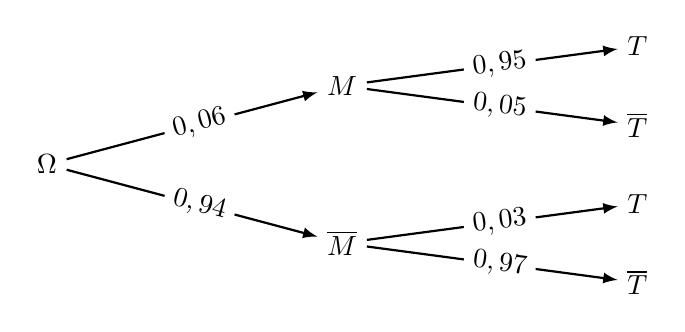
\begin{tikzpicture}[xscale=1,yscale=1]
			\tikzstyle{fleche}=[->,>=latex,thick]
			\tikzstyle{noeud}=[]
			\tikzstyle{etiquette}=[pos=0.53,sloped,fill=white]
			\def\DistanceInterNiveaux{3}
			\def\DistanceInterFeuilles{1}
			\def\NiveauA{(0)*\DistanceInterNiveaux}
			\def\NiveauB{(1.25)*\DistanceInterNiveaux}
			\def\NiveauC{(2.5)*\DistanceInterNiveaux}
			\def\InterFeuilles{(-1)*\DistanceInterFeuilles}
			\node[noeud] (R) at ({\NiveauA},{(1.5)*\InterFeuilles}) {$\Omega$};
			\node[noeud] (Ra) at ({\NiveauB},{(0.5)*\InterFeuilles}) {$M$};
			\node[noeud] (Raa) at ({\NiveauC},{(0)*\InterFeuilles}) {$T$};
			\node[noeud] (Rab) at ({\NiveauC},{(1)*\InterFeuilles}) {$\overline{T}$};
			\node[noeud] (Rb) at ({\NiveauB},{(2.5)*\InterFeuilles}) {$\overline{M}$};
			\node[noeud] (Rba) at ({\NiveauC},{(2)*\InterFeuilles}) {$T$};
			\node[noeud] (Rbb) at ({\NiveauC},{(3)*\InterFeuilles}) {$\overline{T}$};
			\draw[fleche] (R)--(Ra) node[etiquette] {$0,06$};
			\draw[fleche] (Ra)--(Raa) node[etiquette] {$0,95$};
			\draw[fleche] (Ra)--(Rab) node[etiquette] {$0,05$};
			\draw[fleche] (R)--(Rb) node[etiquette] {$0,94$};
			\draw[fleche] (Rb)--(Rba) node[etiquette] {$0,03$};
			\draw[fleche] (Rb)--(Rbb) node[etiquette] {$0,97$};
		\end{tikzpicture}
	\end{center}
	\item On a (probabilités composées) :
	%
	\begin{itemize}
		\item $P(M \cap T) = 0,06 \times 0,95 = 0,057$ ;
		\item $P\big(\overline{M}\cap\overline{T}\big)=0,94\times0,97=\num{0,9118}$ ;
		\item $P\big(\overline{M}\cap T\big)=0,94\times0,03=\num{0,0282}$.
	\end{itemize}
	\item D'après la formule des probabilités totales, $P(T)=P(M \cap T)+P\big(\overline{M}\cap T\big) = 0,057 + \num{0,0282} = \num{0,0852}$.
	\item La probabilité recherchée est $P_T(M)=\dfrac{P(M \cap T)}{P(T)}=\dfrac{0,057}{\num{0,0852}} \approx \num{0,669}$ au millième.
\end{enumerate}

\medskip

\exogen{ B2}

\medskip

Le tableau complété est :
%
\begin{center}
	\begin{tblr}{width=0.8\linewidth,colspec={X[c]X[c]X[c]X[c]},%rows={7mm},
			hline{1}={2-5}{solid,0.8pt},hline{2-5}={solid,0.8pt},
			vline{1}={2-5}{solid,0.8pt},vline{2-5}={solid,0.8pt},
			cell{1}{2,3,4}={lightgray!50},cell{2,3,4}{1}={lightgray!50}
		}
		& \textbf{Malades} & \textbf{Sains} & \textbf{Total} \\
		\textbf{Fumeurs} & 400 & \num{4600} & \num{5000}  \\
		\textbf{Non-Fumeurs} & 600 & \num{14400} & \num{15000} \\
		\textbf{Total} & \num{1000} & \num{19000} & \num{20000} \\
	\end{tblr}
\end{center}

\begin{enumerate}
	\item La probabilité que la personne soit malade est de $\dfrac{1000}{20\,000}=0,05$.
	\item 
	\begin{enumerate}
		\item On a -- par lecture directe -- $p_F(M) = \dfrac{400}{5000}=0,08$.
		\item Cette probabilité représente la probabilité pour une personne d’être malade sachant qu’elle est fumeuse.
	\end{enumerate}
	\item On cherche $p_{\overline{F}} (M) = \dfrac{600}{15\,000}=0,04$.
	\item Le fait de fumer semble être un facteur aggravant car $p_F(M) >  p_{\overline{F}} (M)$.
	
	NB : On peut même parler d’un facteur de risque environ 2 fois plus élevé.
\end{enumerate}

\medskip

\exogen{ B3}

\begin{enumerate}
	\item On peut proposer l'arbre suivant :
	%
	\begin{center}
		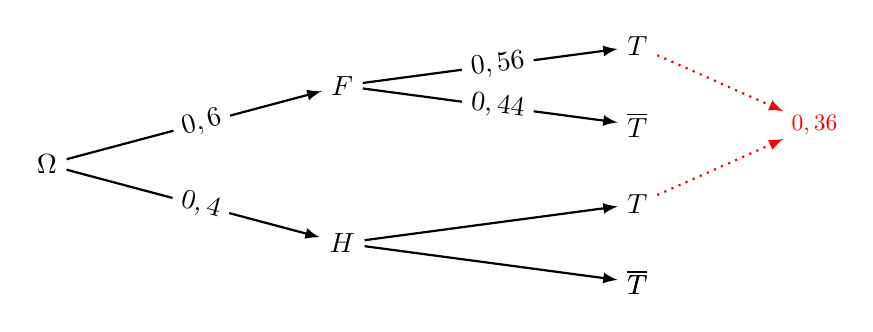
\begin{tikzpicture}[xscale=1,yscale=1]
			\tikzstyle{fleche}=[->,>=latex,thick]
			\tikzstyle{noeud}=[]
			\tikzstyle{finarbre}=[->,dotted,thick,>=latex,color=red]
			\tikzstyle{probinter}=[scale=0.85,color=red]
			\tikzstyle{etiquette}=[pos=0.53,sloped,fill=white]
			\def\DistanceInterNiveaux{3}
			\def\DistanceInterFeuilles{1}
			\def\NiveauA{(0)*\DistanceInterNiveaux}
			\def\NiveauB{(1.25)*\DistanceInterNiveaux}
			\def\NiveauC{(2.5)*\DistanceInterNiveaux}
			\def\NiveauD{(3.25)*\DistanceInterNiveaux}
			\def\InterFeuilles{(-1)*\DistanceInterFeuilles}
			\node[noeud] (R) at ({\NiveauA},{(1.5)*\InterFeuilles}) {$\Omega$};
			\node[noeud] (Ra) at ({\NiveauB},{(0.5)*\InterFeuilles}) {$F$};
			\node[noeud] (Raa) at ({\NiveauC},{(0)*\InterFeuilles}) {$T$};
			\node[noeud] (Rab) at ({\NiveauC},{(1)*\InterFeuilles}) {$\overline{T}$};
			\node[noeud] (Rb) at ({\NiveauB},{(2.5)*\InterFeuilles}) {$H$};
			\node[noeud] (Rba) at ({\NiveauC},{(2)*\InterFeuilles}) {$T$};
			\node[noeud] (Rbb) at ({\NiveauC},{(3)*\InterFeuilles}) {$\overline{T}$};
			\node[noeud] (Rbb) at ({\NiveauC},{(3)*\InterFeuilles}) {$\overline{T}$};
			\node[probinter] (Raaa) at ({\NiveauD},{(1)*\InterFeuilles}) {$0,36$};
			\draw[fleche] (R)--(Ra) node[etiquette] {$0,6$};
			\draw[fleche] (Ra)--(Raa) node[etiquette] {$0,56$};
			\draw[fleche] (Ra)--(Rab) node[etiquette] {$0,44$};
			\draw[fleche] (R)--(Rb) node[etiquette] {$0,4$};
			\draw[fleche] (Rb)--(Rba) ;
			\draw[fleche] (Rb)--(Rbb) ;
			\draw[finarbre] (Raa)--(Raaa) ;
			\draw[finarbre] (Rba)--(Raaa) ;
		\end{tikzpicture}
	\end{center}
	\item On cherche ici $P_T(H)=\dfrac{P(H\cap T)}{P(H)}$ et il nous manque donc $P(H\cap T)$.
	
	D'après la formule des probabilités totales, on a $P(H \cap T) + P(F \cap T) = 0,36 \Rightarrow P(H \cap T) = 0,36 - 0,6 \times 0,56 = 0,024$.
	
	Ainsi $P_T(H)=\dfrac{P(H\cap T)}{P(H)} = \dfrac{0,024}{0,4}=0,06$.
\end{enumerate}

\medskip

\exogen{ B4}

\begin{enumerate}
	\item La somme des probas doit faire 1, donc on obtient $a=1-(0,10+0,05+\ldots+0,10)=0,15$.
	\item 
	\begin{enumerate}
		\item On a $P(X>3)=P(X=4)+\ldots+P(X=8)=0,10+0,20+0,10+0,10+0,15=0,65$.
		\item Et $P(X\pp3) = P(X=0)+P(X=1)+P(X=2)+P(X=3)=0,10+0,05+0,15+0,05=0,35$.
	\end{enumerate}
\end{enumerate}

\medskip

\exogen{ B5}

\begin{enumerate}
	\item On peut utiliser un tableau à double entrée :
	
	\begin{center}
		\begin{tblr}{hlines,vlines,width=5cm,colspec={X[c]X[c]X[c]X[c]X[c]},cells={font=\sffamily},cell{1}{2-5}={blue!10},cell{2-5}{1}={red!10}}
			& 1 & 2 & 3 & 4 \\
			1 & 2 & 3 & 4 & 5 \\
			2 & 3 & 4 & 5 & 6 \\
			3 & 4 & 5 & 6 & 7 \\
			4 & 5 & 6 & 7 & 8 \\
		\end{tblr}
	\end{center}
	
	On obtient donc la loi de probabilités :
	
	\begin{center}
		\begin{tblr}{hlines,vlines,width=11cm,colspec={l*{7}{X[c]}}}
			Valeurs $x_i$ & 2 & 3 & 4 & 5 & 6 & 7 & 8 \\
			Probas $p_i$ & $\nicefrac{1}{16}$ & $\nicefrac{2}{16}$ & $\nicefrac{3}{16}$ & $\nicefrac{4}{16}$ & $\nicefrac{3}{16}$ & $\nicefrac{2}{16}$ & $\nicefrac{1}{16}$ \\
		\end{tblr}
	\end{center}
	\item On calcule $\esp{X}=2 \times \dfrac{2}{16} + 3 \times \dfrac{3}{16} + \ldots + 8 \times \dfrac{1}{16} = 5$.
	
	Sur un très grand nombre de tirages, on peut espérer gagner 5\,€.
\end{enumerate}

\medskip

\exogen{ B6}

\begin{enumerate}
	\item On peut proposer l'arbre suivant :
	%
	\begin{center}
		% Racine à Gauche, développement vers la droite
		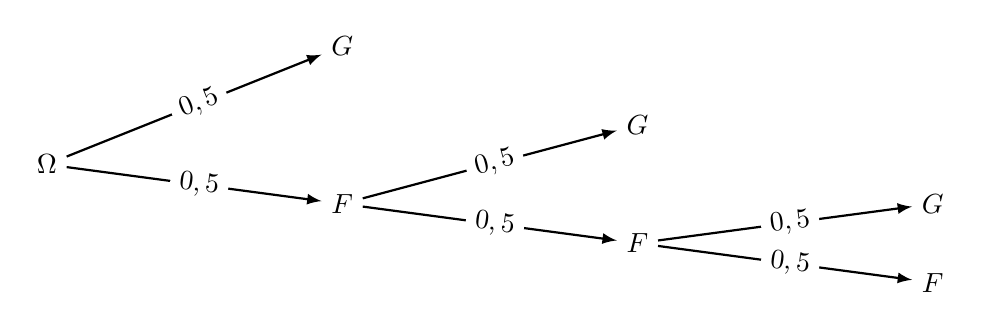
\begin{tikzpicture}[xscale=1,yscale=1]
			\tikzstyle{fleche}=[->,>=latex,thick]
			\tikzstyle{noeud}=[]
			\tikzstyle{etiquette}=[pos=0.52,sloped,fill=white]
			\def\DistanceInterNiveaux{3}
			\def\DistanceInterFeuilles{1}
			\def\NiveauA{(0)*\DistanceInterNiveaux}
			\def\NiveauB{(1.25)*\DistanceInterNiveaux}
			\def\NiveauC{(2.5)*\DistanceInterNiveaux}
			\def\NiveauD{(3.75)*\DistanceInterNiveaux}
			\def\InterFeuilles{(-1)*\DistanceInterFeuilles}
			\node[noeud] (R) at ({\NiveauA},{(1.5)*\InterFeuilles}) {$\Omega$};
			\node[noeud] (Ra) at ({\NiveauB},{(0)*\InterFeuilles}) {$G$};
			\node[noeud] (Rb) at ({\NiveauB},{(2)*\InterFeuilles}) {$F$};
			\node[noeud] (Rba) at ({\NiveauC},{(1)*\InterFeuilles}) {$G$};
			\node[noeud] (Rbb) at ({\NiveauC},{(2.5)*\InterFeuilles}) {$F$};
			\node[noeud] (Rbba) at ({\NiveauD},{(2)*\InterFeuilles}) {$G$};
			\node[noeud] (Rbbb) at ({\NiveauD},{(3)*\InterFeuilles}) {$F$};
			\draw[fleche] (R)--(Ra) node[etiquette] {$0,5$};
			\draw[fleche] (R)--(Rb) node[etiquette] {$0,5$};
			\draw[fleche] (Rb)--(Rba) node[etiquette] {$0,5$};
			\draw[fleche] (Rb)--(Rbb) node[etiquette] {$0,5$};
			\draw[fleche] (Rbb)--(Rbba) node[etiquette] {$0,5$};
			\draw[fleche] (Rbb)--(Rbbb) node[etiquette] {$0,5$};
		\end{tikzpicture}
	\end{center}
	\item Les valeurs prises par $X$ sont 1, 2 ou 3 :
	%
	\begin{itemize}
		\item $P(X=1)=P("\text{1 garçon}")=0,5$ ;
		\item $P(X=2)=P("\text{1 garçon et 1 fille}") = 0,5 \times 0,5 = 0,25$ ;
		\item $P(X=3)=P("\text{2 filles et 1 garçon ou 3 filles}") = 0,5^3 + 0,5^3 = 0,25$.
	\end{itemize}
	%
	On obtient la loi de probabilités :
	
	\begin{center}
		\begin{tblr}{hlines,vlines,width=6cm,colspec={l*{3}{X[c]}}}
			Valeurs $x_i$ & 1 & 2 & 3 \\
			Probas $p_i$ & $0,5$ & $0,25$ & $0,25$ \\
		\end{tblr}
	\end{center}
	\item On a $\esp{X}=1 \times 0,5 + 2 \times 0,25 + 3 \times 0,25 = 1,75$.
	
	Sur la planète Dictat, le nombre moyen d'enfants est de $1,75$.
\end{enumerate}

\pagebreak

\exogen{ C1}

\begin{enumerate}
	\item 
	\begin{enumerate}
		\item Pour les images, on lit la \og hauteur \fg{} de la courbe :
		\begin{itemize}
			\item $f(-3)=3$ ;
			\item $f(2)=2$ ;
			\item $f(6)=-4$.
		\end{itemize}
		\item Pour les nombres dérivés, on lit la \og pente \fg{} des tangentes :
		\begin{itemize}
			\item $f'(-3)=\tfrac{1}{2}=0,5$ ;
			\item $f'(2)=\tfrac{-2}{1}=-2$ ;
			\item $f'(6)=\tfrac{3}{2}=1,5$.
		\end{itemize}
	\end{enumerate}
	\item 
	\begin{enumerate}
		\item On sait que $f'(a)=0$ lorsque $\mathscr{T}_a$ est horizontale, ce qui semble être le cas pour $a=-0,5$ ou $a=5$.
		\item Dans ce cas, la tangente $\mathscr{T}_a$ est horizontale !
	\end{enumerate}
\end{enumerate}

\medskip

\exogen{ C2}

\begin{enumerate}
	\item La fonction $f$ se présente sous la forme d'une somme :
	
	\hspace{0.5cm}$h'(x)=3 \times 4x^3-0,5 \times 2x- \dfrac{-1}{x^2} = 12x^3-x+\dfrac{1}{x^2}$.
	\item La fonction $g$ se présente sous la forme d'un produit :
	
	\hspace{0.5cm}$g'(x)=1 \times \sqrt{x} + \dfrac{1}{2\sqrt{x}} \times x = \sqrt{x} + \dfrac{x}{2\sqrt{x}} = \dfrac{\sqrt{x} \times 2\sqrt{x}}{2\sqrt{x}} + \dfrac{x}{2\sqrt{x}} = \dfrac{2x+x}{2\sqrt{x}}=\dfrac{3x}{2\sqrt{x}}$.
	\item La fonction $h$ se présente sous la forme d'un quotient :
	
	\hspace{0.5cm}$h'(x)=\dfrac{-2\times(x+2)-1\times(-2x-3)}{(x+2)^2}=\dfrac{-2x-4+2x+3}{(x+2)^2}=\dfrac{-1}{(x+2)^2}$.
	\item La fonction $i$ se présente sous la forme d'une composée $u^4$ qui se dérive en $4u'u^3$ :
	
	\hspace{0.5cm}$i'(x)=4 \times (-1) \times (1-x)^3 = -4(1-x)^3$.
\end{enumerate}

\medskip


\exogen{ C3}

\begin{enumerate}
	\item 
	\begin{enumerate}
		\item On a $f'(x)=3\times2x-2=6x-2$ ce qui donne $f'(-1)=6\times(-1)-2=-8$.
		\item De ce fait,  $f'(-1)$ est le coefficient directeur de la tangente à $\mathscr{C}_f$ au point d’abscisse $-1$.
	\end{enumerate}
	\item De plus $\mathscr{T}_{-1}$ : $y=f'(-1) \times (x-(-1)) + f(-1) = -8(x+1) + 6 = -8x-8+6 = -8x-2$.
\end{enumerate}

\medskip

\exogen{ C4}

\begin{enumerate}
	\item La fonction $f$ est dérivable sur $\R$ avec $f'(x)=-3\times2x+2=-6x+2$.
	
	Cette dérivée est une fonction affine, pour laquelle $m=-6\ominus$, et qui s'annule en $x_1=\tfrac{1}{3}$.
	
	\begin{center}
		\begin{tikzpicture}
			\tkzTabInit[]{$x$/0.8,$f'(x)$/0.8,$f$/1.6}{$-\infty$,$\nicefrac{1}{3}$,$+\infty$}
			\tkzTabLine{,+,z,-,}
			\aidesignetkztabPL[code=da-,racines={x1},couleur=orange]{1}[0.75][1.5]
			\tkzTabVar{-/,+/$\nicefrac{4}{3}$,-/}
		\end{tikzpicture}
	\end{center}
	\item La fonction $g$ est dérivable sur $\R$ avec $g'(x)=\dfrac{1}{3} \times 3x^2-\dfrac14 \times 2x - \dfrac32 = x^2-0,5x-1,5$.
	
	Cette dérivée est un trinôme, pour lequel $a=1\oplus$, et $\Delta=6,25$ qui donne les racines $x_1=-1$ et $x_2=1,5$.
	
	\begin{center}
		\begin{tikzpicture}
			\tkzTabInit[]{$x$/0.8,$g'(x)$/0.8,$g$/1.6}{$-\infty$,$-1$,${1,5}$,$+\infty$}
			\tkzTabLine{,+,z,-,z,+,}
			\aidesignetkztabPL[code=pa+d+,racines={-1/1,5},couleur=blue]{1}[0.75][1.5]
			\tkzTabVar{-/,+/$M$,-/$m$,+/}
		\end{tikzpicture}
		
		Avec $M=g(-1)=-\dfrac{37}{12}$ et $m=g(1,5)=-5,6875$.
	\end{center}
\end{enumerate}

\medskip

\exogen{ C5}


\begin{enumerate}
	\item On a $A=\dfrac{\e^{3x} \times \e^{-x}}{\e^x}=\dfrac{\e^{3x-x}}{\e^x}=\dfrac{\e^{2x}}{\e^x}=\e^{2x-x} = \e^{x}$.
	
	Et $B=\e^x \times \big(\e^{-2x}\big)^3 = \e^x \times \e^{3 \times (-2x)} = \e^x \times \e^{-6x} = \e^{x-6x} = \e^{-5x}$.
	\item On a $C=\e^2\left(\e^{-2}+\e\right) = \e^{2-2} + \e^{2+1} = \e^0 + \e^3 = 1 + \e^3$.
	
	Et $D=\big(\e^4-\e\big)\big(\e^4+\e\big) = \e^{4+4}+\e^{4+1}-\e^{1+4}-\e^2 = \e^8 - \e^2$.
	\item On a $E=2\e^{6x}-\e^{2x} = 2\e^{2x+4x} - \e^{2x} = \e^{2x} \big(2\e^{4x}-1\big)$.
\end{enumerate}

\medskip

\exogen{ C6}

\begin{enumerate}
	\item $f(x)=-3\e^x+4\e^{-2x+1}+\e$ se dérive comme une somme, avec une exponentielle composée :
	
	\hspace{5mm}$f'(x)=-3\e^x + 4 \times (-2) \times \e^{-2x+1} = -3\e^x - 8\e^{-2x+1}$.
	\item $g(x)=\big(\e^x+1\big)\big(\e^x-1\big)$ se dérive comme un produit
	
	\hspace{5mm}$g'(x)= \e^x \left(\e^x-1\right) + \e^x \left(\e^x+1\right) = \e^x \left( \e^x-1+\e^x+1 \right) = \e^x \times \left(2\e^x\right) = 2\e^{2x}$.
	\item $h(x)=\dfrac{4}{\e^{-x}}$ se dérive comme un quotient, avec une exponentielle composée :
	
	\hspace{5mm}$h'(x)=\dfrac{0 \times \e^{-x} - \big(-\e^{-x}\big) \times 4}{\big(\e^{-x}\big)^2} = \dfrac{4\e^{-x}}{\e^{-2x}}=4\e^{-x+2x}=4\e^{x}$.
	\item $i(x)=\dfrac{\e^x}{x+1}$ se dérive comme un quotient :
	
	\hspace{5mm}$i'(x)=\dfrac{\e^x \times (x+1) - 1 \times \e^x}{(x+1)^2}=\dfrac{\e^x(x+1-1)}{(x+1)^2}=\dfrac{x\e^x}{\big(\e^x\big)^2} = \dfrac{x}{\e^x}$.
	\item $j(x)=\dfrac{\e^x+1}{\e^x-1}$ se dérive comme un quotient :
	
	\hspace{5mm}$j'(x)=\dfrac{\e^x \times \big(\e^x-1\big)-\e^x \times \big(\e^x+1\big)}{\big(\e^x-1\big)^2}=\dfrac{\e^x \big( \e^x-1-\e^x-1\big)}{\big(\e^x-1\big)^2} = \dfrac{-2\e^x}{\big(\e^x-1\big)^2}$.
\end{enumerate}

\medskip

\exogen{ C7}

\begin{enumerate}
	\item L'ensemble de définition de $\mathscr{V}$ est $\intervFF{0}{2,5}$ (on ne peut enlever \textit{que} $2,5$~m au maximum à chaque coin).
	
	De plus, $\mathscr{V}=\ell \times \ell \times h = (5-2x)\times(5-2x)\times x = (25-20x+4x^2) \times x = 4x^3-20x^2+25x$.
	\item On étudie les variations de $\mathscr{V}$ :
	
	\begin{itemize}
		\item $\mathscr{V}'(x)=12x^2-40x+25$ ;
		\item $\mathscr{V}'(x)$ est un trinôme, avec $\Delta=400$ et les deux racines sont $x_1=\dfrac{5}{6}$ et $x_2=2,5$.
	\end{itemize}
	
	\begin{center}
		\begin{tikzpicture}
			\tkzTabInit[]{$x$/0.8,$\mathscr{V}'(x)$/0.8,$\mathscr{V}$/1.6}{$0$,$\nicefrac{5}{6}$,${2,5}$}
			\tkzTabLine{,+,z,-,z}
			\aidesignetkztabPL[code=pa+d+,racines={x1/x2},couleur=purple]{1}[0.75][1.5]
			\tkzTabVar{-/$0$,+/$M$,-/$0$}
		\end{tikzpicture}
		
		Avec $M=\left(\frac56\right)=\dfrac{250}{27} \approx 9,259$ à $10^{-3}$.
	\end{center}
	\item Les dimensions de la cuve de volume maximal sont (en m, arrondies au centimètre) $3,33 \times 3,33 \times 0,83$ ($5-2x$ et $x$).
\end{enumerate}

\begin{center}
	\begin{tikzpicture}[x=4cm,y=0.5cm,xmin=0,xmax=3,xgrille=1,xgrilles=0.125,ymin=0,ymax=10,ygrille=2,ygrilles=1]
		\tgrilles \tgrillep \axestikz*
		\axextikz{0,0.25,...,2.75} \axeytikz{0,1,...,9}
		%\clip (\xmin,\ymin) rectangle (\xmax,\ymax) ;
		\draw[very thick,red,domain=\xmin:2.5,samples=250] plot (\x,{4*\x*\x*\x-20*\x*\x+25*\x}) ;
		\draw[ForestGreen,very thick] ({5/6},0) -- ({5/6},{250/27}) circle[fill= ForestGreen,radius=2.5pt] -- (0,{250/27}) ;
	\end{tikzpicture}
\end{center}

\exogen{ C8}

\begin{enumerate}
	\item La fonction $f$ est dérivable (somme et produit) sur $\R$ et :
	
	\hspace{5mm}$f'(x)=1 \times \e^x + \e^x \times (x-2) + 1 = \e^x (1+x-2)+1 = \e^x(x-1)+1$.
	\item 
	\begin{enumerate}
		\item La fonction $g$ est dérivable (somme et produit) sur $\R$ et :
		
		\hspace{5mm}$g'(x)= 1 \times \e^x + \e^x \times (x-1) = \e^x (1+x-1) = x\,\e^x$.
		
		On étudie le signe de $g'(x)$, qui s'exprime comme un produit :
		
		\begin{itemize}
			\item $x=0$ et $m=1\oplus$ ;
			\item $\e^x > 0$ !
		\end{itemize}
		
		\begin{center}
			\begin{tikzpicture}
				\tkzTabInit[]{$x$/0.8,$x$/0.8,$\e^x$/0.8,$g'(x)$/0.8,$g$/1.6}{$-\infty$,$0$,$+\infty$}
				\tkzTabLine{,-,z,+,}
				\tkzTabLine{,+,t,+,}
				\tkzTabLine{,-,z,+,}
				\aidesignetkztabPL[code=da+,racines={0},couleur=blue]{1}[0.75][1.5]
				\tkzTabVar{+/,-/$0$,+/}
			\end{tikzpicture}
		\end{center}
		\item D'après le tableau de variations, $g$ admet un minimum égal à $0$ donc $g(x) \pg  0$ pour tout réel $x$.
	\end{enumerate}
	\item On a bien $f'(x) =  g(x)$.
	
	Or on vient de montrer que $g(x)\pg  0$ pour tout réel $x$, donc $f'(x) \pg  0$ pour tout réel $x$.
	
	Ainsi $f$ est strictement croissante sur $\R$ !
\end{enumerate}

\pagebreak

\exogen{ C9}

\begin{enumerate}
	\item On calcule $f(0)=6\times\dfrac{\e^{0}-1}{\e^{0}+1}=6\times\dfrac{1-1}{1+1}=0$, donc pas de vitesse initiale.
	\item 
	\begin{enumerate}
		\item La fonction $f$ est dérivable (quotient et exponentielle composée) et :
		
		\hspace{5mm}$f'(t)=6 \times \dfrac{0,1\e^{0,1t} \times \big(\e^{0,1t}+1\big)-0,1\e^{0,1t}\times\big(\e^{0,1t}-1\big)}{\big(\e^{0,1t}+1\big)^2} = 6 \times \dfrac{0,1\e^{0,2t}+0,1\e^{0,1t}-0,1\e^{0,2t}+0,1\e^{0,1t}}{\big(\e^{0,1t}+1\big)^2}$
		
		\hspace{5mm}$\phantom{f'(t)}= 6 \times \dfrac{0,2\e^{0,1t}}{\big(\e^{0,1t}+1\big)^2} = \dfrac{1,2\e^{0,1t}}{\big(\e^{0,1t}+1\big)^2}$.
		\item On constate que $f'(t)$ est strictement positive (une exponentielle et un carré sont positifs !).
		
		Donc $f$ est croissante sur $\intervFO{0}{+\infty}$.
	\end{enumerate}
\end{enumerate}

\medskip

\exogen{ D1}

\begin{enumerate}
	\item On détermine la mesure principale des angles proposés :
	\begin{multicols}{4}
		\begin{itemize}
			\item $5\pi$ donne $\pi$ ; $\vphantom{-\dfrac{9\pi}{4}}$
			\item $-\dfrac{3\pi}{2}$ donne $\dfrac{\pi}{2}$ ; $\vphantom{-\dfrac{9\pi}{4}}$
			\item $\dfrac{7\pi}{3}$ donne $\dfrac{\pi}{3}$ ; $\vphantom{-\dfrac{9\pi}{4}}$
			\item $-\dfrac{9\pi}{4}$ donne $-\dfrac{\pi}{4}$. $\vphantom{-\dfrac{9\pi}{4}}$
		\end{itemize}
	\end{multicols}
	\begin{center}
		\begin{tikzpicture}[line join=bevel]
			\cercletrigoPL[rayon=2.5,affangles=false,taillevaleurs=\tiny]
			\filldraw[ForestGreen] (180:2.5) circle[radius=2.5pt] node[above left,font=\scriptsize] {$5\pi$} ;
			\filldraw[orange] (90:2.5) circle[radius=2.5pt] node[above left,font=\scriptsize] {$-\dfrac{3\pi}{2}$} ;
			\filldraw[purple] (60:2.5) circle[radius=2.5pt] node[above right,font=\scriptsize] {$\dfrac{7\pi}{3}$} ;
			\filldraw[blue] (-45:2.5) circle[radius=2.5pt] node[below right,font=\scriptsize] {$-\dfrac{9\pi}{4}$} ;
	\end{tikzpicture}
	\end{center}
	\item En \og enlevant des tours \fg, on obtient $\dfrac{123\pi}{6}=\dfrac{41\pi}{2} = \dfrac{\pi}{2} + 5\times2\pi$ ; donc une mesure principale de $\dfrac{123\pi}{6}$ est $\dfrac{\pi}{2}$.
\end{enumerate}

\medskip

\exogen{ D2}

\begin{multicols}{3}
	\begin{enumerate}
			\item $\cos\left( \dfrac{3\pi}{4}\right) = -\dfrac{\sqrt{2}}{2}$ ;
			\item $\cos\left( -\dfrac{\vphantom{1}\pi}{6}\right) = \dfrac{\sqrt{3}}{2}$ ;
			\item $\cos\left( \dfrac{9\pi}{2}\right) = \cos\left( \dfrac{\pi}{2}\right) = 0$ ;
			\item $\cos\left( -\dfrac{11\pi}{3}\right) = \cos\left( \dfrac{\pi}{3}\right) = \dfrac12$ ;
			\item $\cos\left( \dfrac{5\pi}{6}\right) = -\dfrac{\sqrt{3}}{2}$ ;
			\item $\sin\left( -\dfrac{3\pi}{2}\right) = \sin\left( \dfrac{\pi}{2}\right) = 1$ ;
			\item $\sin\left( \dfrac{5\pi}{3}\right) = \sin\left( -\dfrac{2\pi}{3}\right) = -\dfrac{\sqrt{3}}{2}$ ;
			\item $\sin\left( -\dfrac{\vphantom{1}\pi}{4}\right) = -\dfrac{\sqrt{2}}{2}$ ;
			\item $\sin\left( \dfrac{7\pi}{6}\right) = \sin\left( -\dfrac{5\pi}{6}\right) = -\dfrac12$.
		\end{enumerate}
\end{multicols}

\medskip

\exogen{ D3}

\begin{enumerate}
	\item On a $\vect{u}\cdot\vect{v}=1 \times 6 + (-2) \times 3 = 6 - 6 = 0$, donc $\vect{u}$ et $\vect{v}$ sont orthogonaux.
	\item On a $\vect{w}\cdot\vect{t}=\sqrt{2} \times 2\sqrt{2} + (-1) \times (-4) = 4 + 4 = 8 \neq 0$, donc $\vect{w}$ et $\vect{t}$ ne sont pas orthogonaux.
	\item $\vect{t_1} \perp \vect{t_2} \ssi \vect{t_1}\cdot\vect{t_2} = 0 \ssi 3 \times 6 +a \times (-a) = 0 \ssi 18 -a^2 = 0 \ssi a^2=18 \ssi a=\pm \sqrt{18} = \pm 3\sqrt{2}$.
\end{enumerate}

\pagebreak

\exogen{ D4}

\medskip

On passe par les vecteurs $\begin{dcases} \vect{AB} \begin{pmatrix} 8-5 \\ -5-3 \end{pmatrix} = \begin{pmatrix} 3 \\ -8 \end{pmatrix} \\ \vect{CD} \begin{pmatrix} 3-(-1) \\ 1,5-0 \end{pmatrix} = \begin{pmatrix} 4 \\ 1,5 \end{pmatrix} \end{dcases}$.

\smallskip

Et $\vect{AB}\cdot\vect{CD}=3 \times 4 + (-8) \times 1,5 = 12 - 12 = 0$ ; donc $\vect{AB} \perp \vect{CD}$, et de ce fait $(AB)$ et $(CD)$ sont perpendiculaires.

\bigskip

\exogen{ D5}

\begin{enumerate}
	\item On a $\vect{AB}\cdot\vect{AD} = \begin{pmatrix} 1 \\ -4 \end{pmatrix} \cdot \begin{pmatrix} 4 \\ 1 \end{pmatrix} = 1 \times 4 + (-4) \times 1 = 0$.
	\item 
	\begin{enumerate}
		\item On a $AB = \sqrt{1^2+(-4)^2}=\sqrt{17}$ et $AD = \sqrt{4^2+1^2}=\sqrt{17}$.
		\item Sachant que $\vect{AB}\cdot\vect{AD} = 0$, on en déduit directement que $\widehat{DAB}=90^{\circ}$.
	\end{enumerate}
	\item La quadrilatère $ABCD$ est un losange ($\vect{AD}=\vect{BC}$ et $AB=AD$) avec un angle droit, c'est donc un carré !
\end{enumerate}

\medskip

\exogen{ D6}

\begin{enumerate}
	\item On sait qu'une équation cartésienne de $(d)$ est $-3x+y+c=0$, et $-3\times4+2+c=0 \ssi c=10$.
	
	Ainsi une équation cartésienne est $-3x+y+10=0$.
	\item Un vecteur directeur de $(d')$ est directement $\begin{pmatrix} 1,5 \\ 3 \end{pmatrix}$, qui est colinéaire à $\begin{pmatrix} -4,5 \\ -9 \end{pmatrix}$.
	
	De ce fait, le vecteur $\vect{v}$ est bien directeur de $(d')$.
\end{enumerate}

\medskip

\exogen{ D7}

\begin{enumerate}
	\item On a déjà $y=-4x+5 \ssi 4x+y-5=0$ . Donc un vecteur $\vect{u}$ directeur de $(d)$ a pour coordonnées $\begin{pmatrix} 1 \\ -4 \end{pmatrix}$.
	\item De même, un vecteur $\vect{n}$ normal à $(d)$ a pour coordonnées $\begin{pmatrix} 4 \\ 1 \end{pmatrix}$
	\item $(d')$ sera dirigée par $\vect{n}$, et donc aura pour équation cartésienne $ x-4y+c=0$, avec $1 - 4 \times 1 + c = 0 \ssi c = 3$.
	
	Ainsi une équation cartésienne de $(d')$ est $x - 4y + 3 = 0$.
	\item $x - 4y + 3 = 0 \ssi 4y=x+3 \ssi y=\tfrac{1}{4}x+\tfrac{3}{4}$ est l'équation réduite de $(d')$.
\end{enumerate}

\medskip

\exogen{ D8}

\begin{enumerate}
	\item 
	\begin{enumerate}
		\item $d_1$ : $-3x + 2y + 1 = 0$ admet comme vecteur normal $\vect{n_1} \begin{pmatrix} -3 \\2 \end{pmatrix}$ ;
		\item $d_2$ : $5x + y - 6 = 0$ admet comme vecteur normal $\vect{n_2} \begin{pmatrix} 5 \\1 \end{pmatrix}$ ;
		\item $d_3$ : $y=-2x+4 \ssi 2x+y-4=0$ admet comme vecteur normal $\vect{n_3} \begin{pmatrix} 2 \\1 \end{pmatrix}$ ;
		\item $d_4$ : $x=1 \ssi x-1=0$ admet comme vecteur normal $\vect{n_4} \begin{pmatrix} 1 \\0 \end{pmatrix}$ (droite verticale).
	\end{enumerate}
	\item 
	\begin{enumerate}
		\item La droite aura pour équation cartésienne $1x - 3y + c = 0$ avec $1 \times 4 - 3 \times 1 + c = 0 \ssi c = -1$.
		
		Donc la droite a pour équation cartésienne $x -3y - 1 = 0$
		\item La droite aura pour équation cartésienne $4x + 2y + c = 0$ avec $4 \times 2 + 2 \times 3 + c = 0 \ssi c = −14$.
		
		Donc la droite a pour équation cartésienne $4x + 2y - 14 = 0$.
		\item La droite aura pour équation cartésienne $-3x -1y + c = 0$ avec $-3 \times (-2) - 1 \times (-1) + c = 0 \ssi c = -7$.
		
		Donc la droite a pour équation cartésienne $-3x - y - 7 = 0$.
		\item La droite aura pour équation cartésienne $5x + 3y + c = 0$ avec $5 \times  0 + 3 \times 5 + c = 0 \ssi c = -15$.
		
		Donc la droite a pour équation cartésienne $5x + 3y - 15 = 0$.
	\end{enumerate}
\end{enumerate}

\medskip

\exogen{ D9}

\begin{enumerate}
	\item 
	\begin{enumerate}
		\item On sait qu'un équation cartésienne est $(x-5)^2+(y-4)^2=2^2$.
		
		Soit encore $x^2-10x+25+y^2-8y+16=4 \ssi x^2+y^2-10x-8y+37=0$.
		\item Une équation cartésienne est $(x-(-2))^2+(y-(-3))^2=5^2$.
		
		Soit encore $x^2+4x+4+y^2+6y+9=25 \ssi x^2+y^2+4x+6y-12=0$
	\end{enumerate}
	\item 
	\begin{enumerate}
		\item Dans $(x-2)^2+(y+1)^2=25$, on reconnaît le cercle de centre $\Omega(2\,;\,-1)$ et de rayon $R=\sqrt{25}=5$.
		\item Par \og formes canoniques \fg, on a :
		
		$x^2+y^2-4x+5y+3=0 \ssi x^2-4x+y^2+5y=-3 \ssi (x-2)^2-4 + (y+2,5)^2-6,25=-3$.
		
		Soit encore $(x-2)^2 + (y+2,5)^2=7,25$.
		
		On reconnaît le cercle de centre $\Omega(2\,;\,-2,5)$ et de rayon $R=\sqrt{7,25}$.
	\end{enumerate}
\end{enumerate}

\medskip

\exogen{ E1}

\medskip

\cpy{evolu(750)} va renvoyer le plus petit entier $n$ tel que $u_n \pg 750$ avec $\begin{dcases} u_0 = 200 \\ u_{n+1} = 1,2u_n + 10 \end{dcases}$.

D'après la calculatrice, $\left. \begin{dcases} u_{4} = 675,76 \\ u_{5} = 820,912 \end{dcases} \right| \Rightarrow n \pg 5$ ; et donc \cpy{evolu(750)} renvoie \cpy{5}.

\bigskip

\exogen{ E2}

\medskip

On peut proposer :

\begin{envcodepythontex}[largeur=8cm,lignes,centre=true]
	def Suite() :
		S = 0
		U = 400
		for i in range(20) :
			S = S + U
			U = 0.9*U + 60
		return S
\end{envcodepythontex}

\medskip

\exogen{ E3}

\begin{enumerate}
	\item On a le tableau d'exécution suivant :
	%
	\begin{center}
		\begin{tblr}{width=0.95\linewidth,vlines,hlines,colspec={c*{8}{X[c]}},cells={font=\scriptsize\ttfamily}}
			C 					& 300	& 326	& 338 	& 354.2	& 368.78	& 381.902	& 393.7118	& 404.34062 \\
			\og C < 400 \fg{} ?	& oui	& oui 	& oui	& oui	& oui		& oui		& oui		& non		\\
		\end{tblr}
	\end{center}
	\item De ce fait, la valeur de \cpy{N} renvoyée par ce programme est \cpy{7}.
	
	Concrètement, le nombre de colonies sera supérieur à 400 au bout de 7 ans.
\end{enumerate}

\pagebreak

\exogen{ F1}

\medskip

On peut proposer, avec notamment le \ccalg{ZoomAuto} :

\begin{center}
	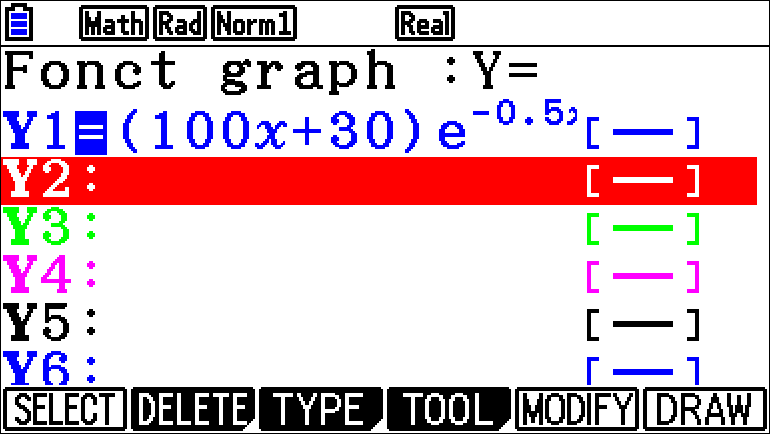
\includegraphics[height=\htimg]{tp01_corr_situ3_a}~~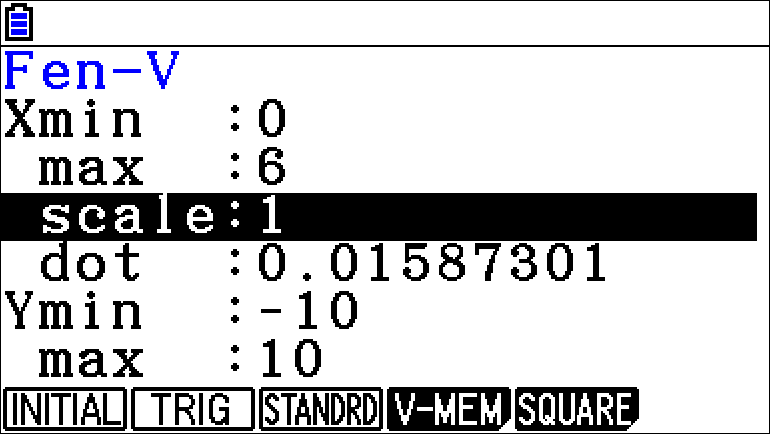
\includegraphics[height=\htimg]{tp01_corr_situ3_b}~~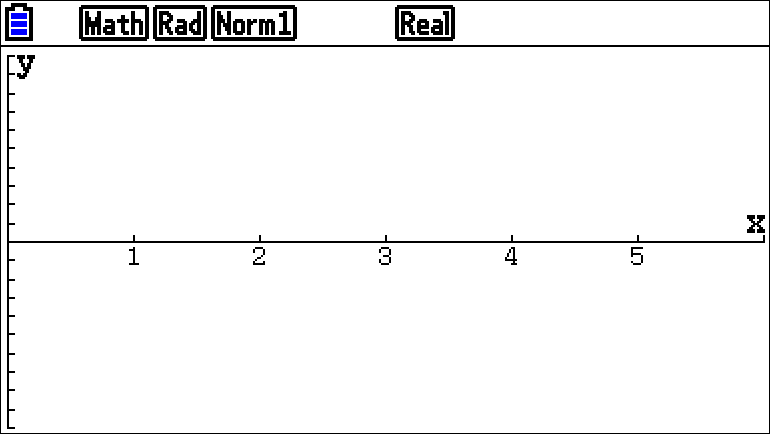
\includegraphics[height=\htimg]{tp01_corr_situ3_c}~~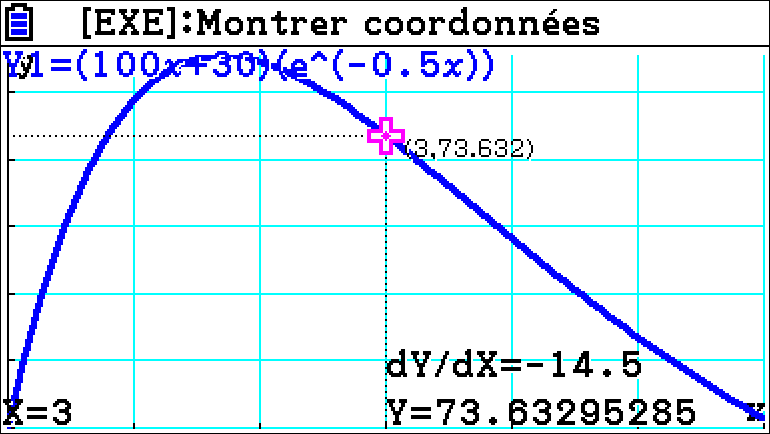
\includegraphics[height=\htimg]{tp01_corr_situ3_d}
\end{center}

\medskip

\exogen{ F2}

\begin{enumerate}
	\item On peut proposer, avec notamment le \ccalg{ZoomAuto} :
	%
	\begin{center}
		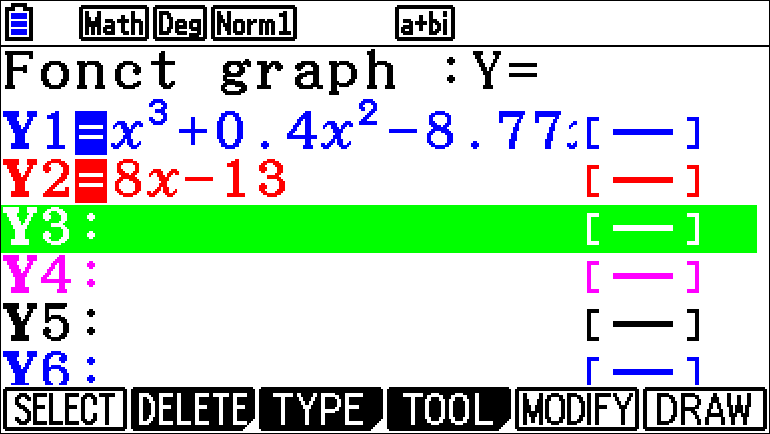
\includegraphics[height=\htimg]{tp01_corr_situ1_a}~~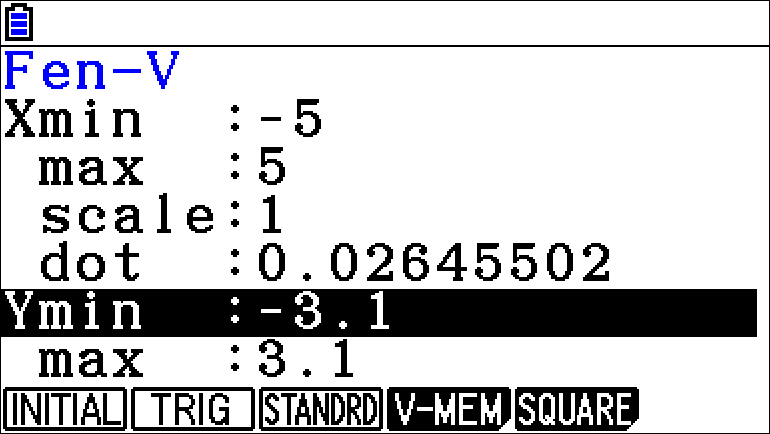
\includegraphics[height=\htimg]{tp01_corr_situ1_b}~~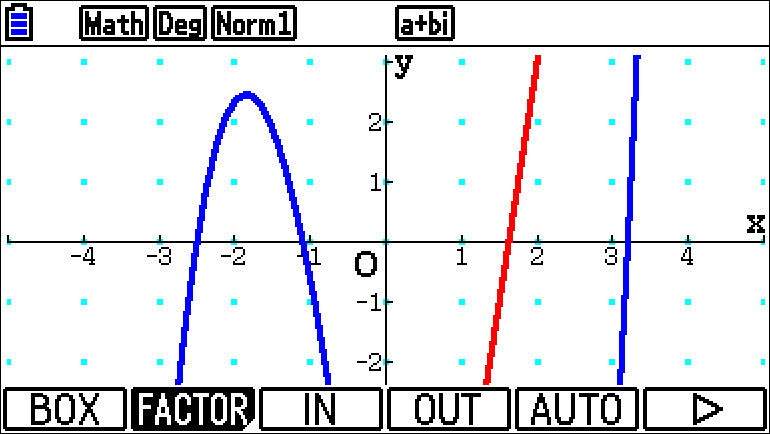
\includegraphics[height=\htimg]{tp01_corr_situ1_c}~~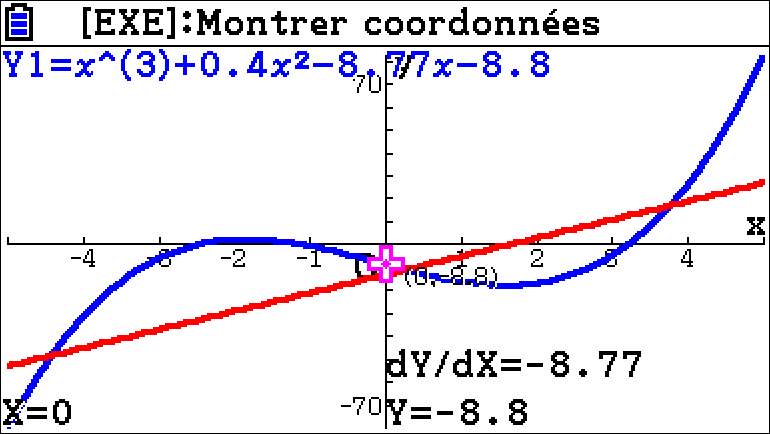
\includegraphics[height=2.15cm]{tp01_corr_situ1_d}
	\end{center}
	\item 
	\begin{enumerate}
		\item les racines sont \ccalg{X=-2.5} ou \ccalg{X=-1.1} ou \ccalg{X=3.2} ;
		\item la solution est \ccalg{X=4.3121} ;
		\item les solutions sont \ccalg{X=-4.4144} ou \ccalg{X=0.25293} ou \ccalg{X=3.76149}.
	\end{enumerate}
\end{enumerate}

\medskip

\exogen{ F3}

\begin{enumerate}
	\item On peut proposer, avec notamment le \ccalg{ZoomAuto} :
	\begin{center}
		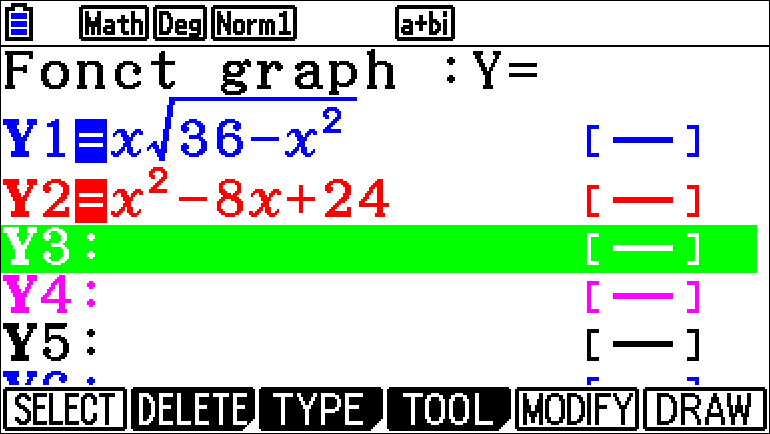
\includegraphics[height=\htimg]{tp01_corr_situ2_a}~~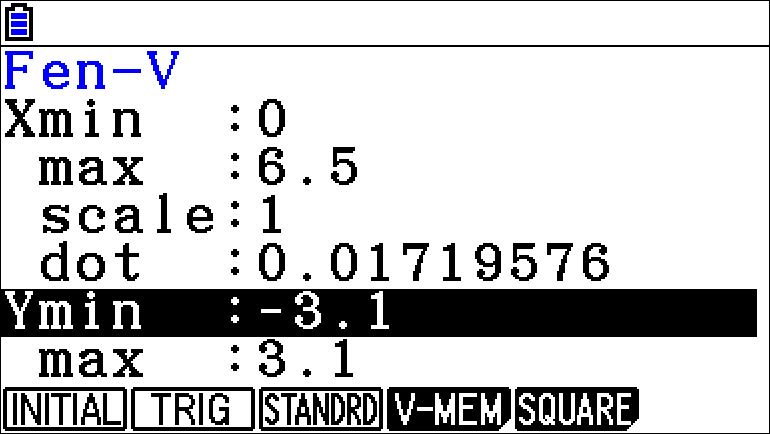
\includegraphics[height=\htimg]{tp01_corr_situ2_b}~~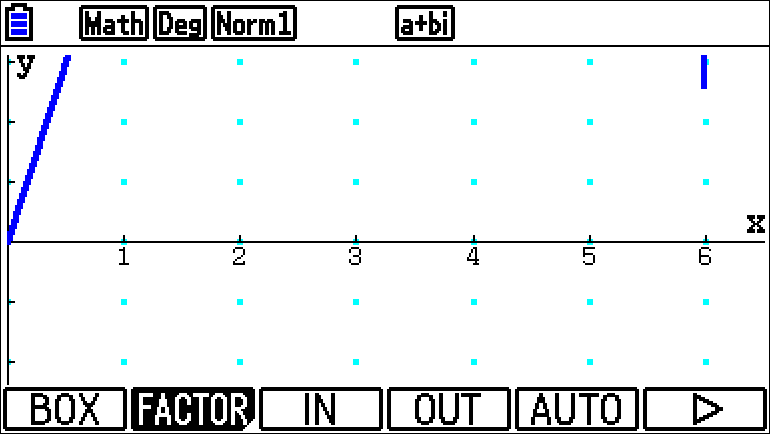
\includegraphics[height=\htimg]{tp01_corr_situ2_c}~~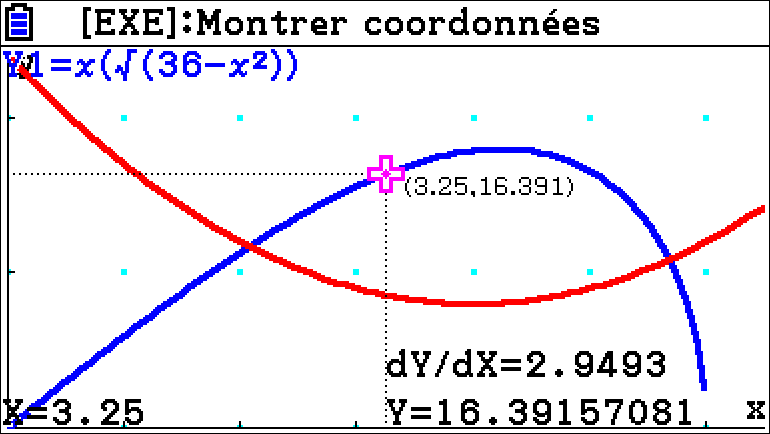
\includegraphics[height=\htimg]{tp01_corr_situ2_d}
	\end{center}
	\item 
	\begin{enumerate}
		\item e maximum est \ccalg{MAX=18} atteint pour \ccalg{X=4.2426} ;
		\item les solutions sont \ccalg{X=1.74166} ou \ccalg{X=5.74166} ;
		\item les solutions sont \ccalg{X=2.0777} ou \ccalg{X=5.6887} ;
		\item la valeur est \ccalg{$\lmoustache$f(x)=59.8390}.
	\end{enumerate}
\end{enumerate}
%
%\begin{cexercice}[ D2 : valeurs de cosinus et sinus]
%Grâce au cercle trigonométrique, déterminer les valeurs suivantes :
%\vspace{-0.5\baselineskip}
%\begin{multicols}{3}
%	\begin{enumerate}
%		\item $\cos\left( \dfrac{3\pi}{4}\right)$ ;
%		\item $\cos\left( -\dfrac{\vphantom{1}\pi}{6}\right)$ ;
%		\item $\cos\left( \dfrac{9\pi}{2}\right)$ ;
%		\item $\cos\left( -\dfrac{11\pi}{3}\right)$ ;
%		\item $\cos\left( \dfrac{5\pi}{6}\right)$ ;
%		\item $\sin\left( -\dfrac{3\pi}{2}\right)$ ;
%		\item $\sin\left( \dfrac{5\pi}{3}\right)$ ;
%		\item $\sin\left( -\dfrac{\vphantom{1}\pi}{4}\right)$ ;
%		\item $\sin\left( \dfrac{7\pi}{6}\right)$.
%	\end{enumerate}
%\end{multicols}
%\vspace*{0pt}
%\end{cexercice}
%
%\begin{cexercice}[ D3 : produit scalaire et vecteurs orthogonaux]
%On considère un repère orthonormé du plan.
%%
%\begin{enumerate}[]
%	\item Montrer que $\vect{u} \coordeux{1}{-2}$ et $\vect{v} \coordeux{6}{3}$ sont orthogonaux. Justifier.
%	\item $\vect{w} \coordeux{\sqrt{2}}{-1}$ et $\vect{t} \coordeux{2\sqrt{2}}{-4}$ sont-ils orthogonaux ? Justifier.
%	\item Déterminer les éventuelles valeurs réelles de $a$ pour que $\vect{t_1} \coordeux{3}{a}$ et $\vect{t_2} \coordeux{6}{-a}$ soient orthogonaux.
%\end{enumerate}
%\end{cexercice}
%
%\begin{cexercice}[ D4 : droites perpendiculaires et produit scalaire (méthode analytique)]
%Dans un repère orthonormé du plan, on donné $A(5\,;\,3)$, $B(8\,;\,-5)$, $C(-1\,;\,0)$ et $D(3\,;\,1,5)$.
%
%Montrer que $(AB)$ et $(CD)$ sont perpendiculaires.
%\end{cexercice}
%
%\begin{cexercice}[ D5 : produit scalaire et nature de quadrilatère]
%Dans le plan muni d’un repère $\Rij$ orthonormé, on considère les quatre points $A(-3\,;\,2)$ ; $B(-2\,;\,-2)$ ; $C(2\,;\,-1)$ et $D(1\,;\,3)$.
%%
%\begin{enumerate}[]
%	\item Déterminer la valeur de $\vect{AB}\cdot\vect{AD}$.
%	\item 
%	\begin{enumerate}
%		\item Calculer les longueurs $AB$ et $AD$.
%		\item Déterminer une valeur approchée au dixième de degré, de l'angle $\widehat{DAB}$.
%	\end{enumerate}
%	\item Démontrer que le quadrilatère $ABCD$ est un rectangle.
%\end{enumerate}
%\end{cexercice}
%
%\begin{cexercice}[ D6 : équations cartésiennes et vecteur directeur]
%\vspace{-0.8\baselineskip}
%\begin{enumerate}[leftmargin=*]
%	\item Soit $(d)$ la droite passant par $A(4\,;\,2)$ et de vecteur directeur $\vect{u}\coordeux{1}{-3}$. Déterminer une éq. cartésienne de $(d)$.
%	\item Soit $(d')$ la droite d’éq. cartésienne $3x - 1,5y + 1 = 0$. Le vecteur $\vect{v} \coordeux{-4,5}{-9}$ est-il un vecteur directeur de $(d')$ ?
%\end{enumerate}
%\end{cexercice}
%
%\begin{cexercice}[ D7 : droite, vecteurs directeurs et normaux, équations cartésiennes et réduites]
%On considère la droite $d$ d’équation réduite $y = -4x + 5$.
%%
%\begin{enumerate}
%	\item Donner un vecteur directeur de $d$.
%	\item En déduire un vecteur normal de $d$.
%	\item Donner une équation cartésienne de la droite $d'$ perpendiculaire à $d$ passant par le point $A(1\,;\,1)$.
%	\item Donner une équation réduite de la droite $d'$.
%\end{enumerate}
%\end{cexercice}
%
%\begin{cexercice}[ D8 : vecteur normal et équation cartésienne de droite]
%\vspace{-0.8\baselineskip}
%\begin{enumerate}[leftmargin=*]
%	\item Donner un vecteur normal de chacune des droites suivantes :
%	\begin{enumerate}
%		\item $d_1$ : $-3x + 2y + 1 = 0$ ;
%		\item $d_2$ : $5x + y - 6 = 0$ ;
%		\item $d_3$ : $y=-2x+4$ ;
%		\item $d_4$ : $x=1$.
%	\end{enumerate}
%	\item Dans chacun des cas, donner une équation cartésienne de la droite passant par $A$ et de vecteur normal $\vect{n}$.
%	\begin{enumerate}
%		\item $A(4\,;\,1)$ et $\vect{n} \coordeux{1}{-3}$ ;
%		\item $A(2\,;\,3)$ et $\vect{n} \coordeux{4}{2}$ ;
%		\item $A(-2\,;\,-1)$ et $\vect{n} \coordeux{-3}{-1}$ ;
%		\item $A(0\,;\,5)$ et $\vect{n} \coordeux{5}{3}$.
%	\end{enumerate}
%\end{enumerate}
%\end{cexercice}
%
%\begin{cexercice}[ D9 : équation cartésienne de cercle]
%\vspace{-0.8\baselineskip}
%\begin{enumerate}[leftmargin=*]
%	\item Déterminer une équation cartésienne :
%	\begin{enumerate}
%		\item du cercle de centre $\Omega(5\,;\,4)$ et de rayon $R=2$ ;
%		\item du cercle de centre $\Omega(-2\,;\,-3)$ et de rayon $R=5$.
%	\end{enumerate}
%	\item Dans chacun des cas, donner le centre et le rayon du cercle dont on donne une équation cartésienne :
%	\begin{enumerate}
%		\item $(x-2)^2+(y+1)^2=25$ ;
%		\item $x^2+y^2-4x+5y+3=0$.
%	\end{enumerate}
%\end{enumerate}
%\end{cexercice}
%
%\pagebreak
%
%\section{Algorithmes}
%
%\begin{cexercice}[ E1 : avec un seuil]
%On considère la fonction \calgpython{} suivante :
%
%\begin{envcodepythontex}[largeur=8cm,lignes,centre=true]
%	def evolu(k):
%		u = 200
%		n = 0
%		while u < k :
%			u = 1.2*u + 10
%			n = n+1
%		return n
%\end{envcodepythontex}
%
%Que renvoie l'appel \cpy{evolu(750)} ?
%\end{cexercice}
%
%\begin{cexercice}[ E2 : avec une somme]
%Soit la suite $\left(u_n\right)$ de premier terme $u_0= 400$ vérifiant la relation, pour tout entier naturel $n$, $u_{n+1} = 0,9u_n +60$.
%
%Compléter la fonction \cpy{Suite} suivante écrite en \calgpython{} qui permet de calculer la somme $S$ des 20 premiers termes de la suite $\left(u_n\right)$.
%
%\begin{envcodepythontex}[largeur=8cm,lignes,centre=true]
%	def Suite() :
%		S = 0
%		for i in range(20) :
%			S = ...............
%			U = ...............
%		return ...
%\end{envcodepythontex}
%\end{cexercice}
%
%\begin{cexercice}[ E3 : en contexte]
%Un apiculteur souhaite étendre son activité de production de miel à une nouvelle région.
%
%Au printemps 2019, il achète $300$ colonies d’abeilles qu’il installe dans cette région.
%
%Il consulte les services spécialisés de la région et s’attend à perdre 8\,\% des colonies chaque hiver. Pour maintenir son activité et la développer, il prévoit d’installer 50 nouvelles colonies chaque printemps, à partir de l’année suivante.
%
%On donne le programme suivant écrit en langage \calgpython{} :
%\begin{envcodepythontex}[largeur=8cm,lignes,centre=true]
%	def algo() :
%		C = 300
%		N = 0
%		while C < 400 :
%			C = C*0.92+50
%			N = N+1
%		return(N)
%\end{envcodepythontex}
%
%\begin{enumerate}
%	\item Recopier et compléter (en arrondissant à l'entier le plus proche) en ajoutant des colonnes, le tableau ci-dessous qui reproduit l’avancement du programme pas à pas :
%	
%	\begin{center}
%		\begin{tblr}{hlines,colspec={|Q[c,3cm]|Q[c,2cm]|Q[c,2cm]|Q[c,2cm]|Q[c,2cm]},cells={font=\ttfamily}}
%		C 					&300	& 326	& \dotfill 	& \\
%		\og C < 400 \fg{} ?	& oui	& oui 	& \dotfill	& \\
%	\end{tblr}
%	\end{center}
%	\item Quelle est la valeur de \cpy{N} renvoyée par le programme ? Interpréter cette valeur dans le contexte de l’exercice.
%\end{enumerate}
%\end{cexercice}
%
%\pagebreak
%
%\section{Utilisation de la calculatrice}
%
%\begin{cexercice}[ F1 : tracé]
%Dans un repère adapté, tracer -- à la calculatrice -- la courbe représentative de la fonction $f$ définie sur $\intervFF{0}{6}$ par $f(x)=(100x+30)\e^{-0,5x}$ .
%\end{cexercice}
%
%
%\begin{cexercice}[ F2 : tracé et outils graphiques, v1]
%On considère les fonctions $f(x)=x^3+0,4x^2-8,77x-8,8$ et $g(x)=8x-13$ définies sur $\intervFF{-5}{5}$.
%%
%\begin{enumerate}
%	\item Dans un repère adapté, tracer -- à la calculatrice -- les courbes $\courbe{f}$ et $\courbe{g}$ de manière à obtenir une fenêtre comme ci-dessous :
%	\begin{center}
%		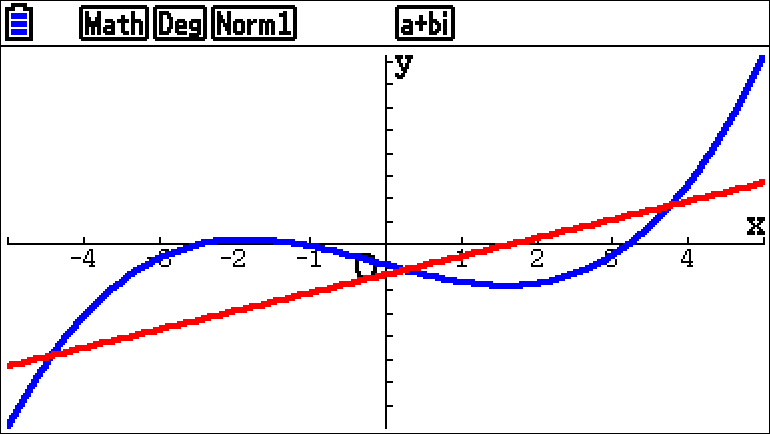
\includegraphics[height=3cm]{tp01_calco_a}
%	\end{center}
%	\item En utilisant les \ccalg{outils graphiques} de la calculatrice :
%	\begin{enumerate}
%		\item déterminer les racines de $f$ (autrement dit les solutions de $f(x)=0$) ;
%		\item déterminer les solutions de $f(x)=41$ ;
%		\item déterminer les solutions de $f(x)=g(x)$.
%	\end{enumerate}
%\end{enumerate}
%\end{cexercice}
%
%\begin{cexercice}[ F3 : tracé et outils graphiques, v2]
%On considère les fonctions $f(x)=x\sqrt{36-x^2}$ et $g(x)=x^2-8x+24$ définies sur $\intervFF{0}{6,5}$.
%%
%\begin{enumerate}
%	\item Dans un repère adapté, tracer -- à la calculatrice -- les courbes $\courbe{f}$ et $\courbe{g}$ de manière à obtenir une fenêtre comme ci-dessous :
%	\begin{center}
%		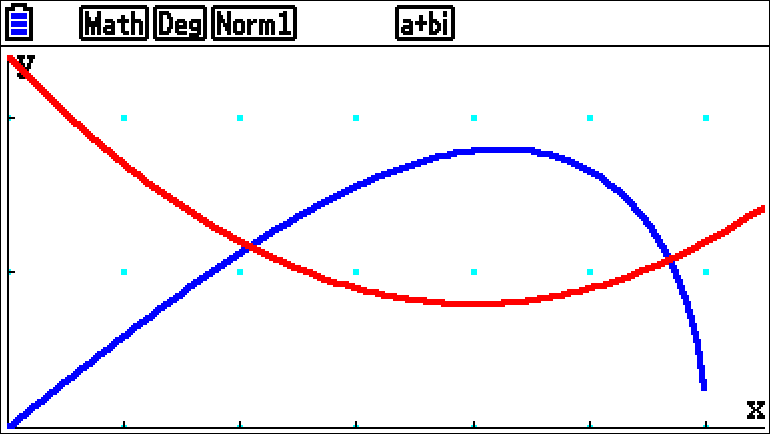
\includegraphics[height=3cm]{tp01_calco_b}
%	\end{center}
%	\item En utilisant les \ccalg{outils graphiques} de la calculatrice :
%	\begin{enumerate}
%		\item déterminer le maximum de $f$, ainsi que la valeur de $x$ pour laquelle il est atteint ;
%		\item déterminer les solutions de $f(x)=10$ ;
%		\item déterminer les solutions de $f(x)=g(x)$ ;
%		\item la valeur de $\int_0^5 f(x) \dx$.
%	\end{enumerate}
%\end{enumerate}
%\end{cexercice}
%
%\vfill{}
%
%\hfill{}{\footnotesize \blue \itshape Largement inspiré du travail d'Alexandre Morgan}

\end{document}